% main.tex -- ARSO 2027 submission (double-blind, 6 pages including references).
% Build: pdflatex main && bibtex main && pdflatex main && pdflatex main
% Local font fallback (must come before \documentclass). The local TeX Live lacks
% texlive-fonts-recommended, so the Times, Helvetica and Courier metrics that IEEEtran
% selects are missing and every glyph would be dropped. txfonts.sty ships with that
% collection, so its absence marks a machine without Times; there the IEEE families are
% silently mapped to Computer Modern. CM is wider than Times, so a local build runs a few
% percent LONGER than the submission build and its page count is conservative.
% On a full TeX Live (or Overleaf) this block does nothing.
\def\CMfallbackfamily#1#2{%
    \DeclareFontFamily{OT1}{#1}{}%
    \DeclareFontShape{OT1}{#1}{m}{n}{<->ssub*#2/m/n}{}%
    \DeclareFontShape{OT1}{#1}{m}{it}{<->ssub*#2/m/it}{}%
    \DeclareFontShape{OT1}{#1}{m}{sl}{<->ssub*#2/m/sl}{}%
    \DeclareFontShape{OT1}{#1}{m}{sc}{<->ssub*#2/m/sc}{}%
    \DeclareFontShape{OT1}{#1}{b}{n}{<->ssub*#2/bx/n}{}%
    \DeclareFontShape{OT1}{#1}{bx}{n}{<->ssub*#2/bx/n}{}%
    \DeclareFontShape{OT1}{#1}{b}{it}{<->ssub*#2/bx/it}{}%
    \DeclareFontShape{OT1}{#1}{bx}{it}{<->ssub*#2/bx/it}{}%
    \DeclareFontShape{OT1}{#1}{b}{sl}{<->ssub*#2/bx/sl}{}%
    \DeclareFontShape{OT1}{#1}{bx}{sl}{<->ssub*#2/bx/sl}{}%
    \DeclareFontShape{OT1}{#1}{b}{sc}{<->ssub*#2/m/sc}{}%
    \DeclareFontShape{OT1}{#1}{bx}{sc}{<->ssub*#2/m/sc}{}}
\IfFileExists{txfonts.sty}{}{%
  \CMfallbackfamily{ptm}{cmr}\CMfallbackfamily{phv}{cmss}\CMfallbackfamily{pcr}{cmtt}%
  \typeout{*** main.tex: Times metrics not installed; IEEE fonts mapped to Computer Modern (page count is conservative). ***}%
}
\documentclass[conference]{IEEEtran}


\usepackage{amsmath}
\usepackage{amssymb}
\usepackage{graphicx}
\usepackage{cite}
\usepackage{booktabs}
\usepackage{xcolor}
% TikZ (pgf) is not installed in the local TeX Live (texlive-pictures missing), so it is
% loaded only when present. Fig. 1 is drawn with the built-in picture environment and
% does not need it. Do not use TikZ in the section files.
\IfFileExists{tikz.sty}{%
  \usepackage{tikz}%
  \usetikzlibrary{arrows.meta,positioning,fit}%
}{}

% Anonymous PDF metadata (no hyperref). Also drop pdfTeX's file-path and date entries.
\ifdefined\pdfinfo
  \pdfinfo{/Title () /Author () /Subject () /Keywords () /Creator ()}
  \pdfinfoomitdate=1
  \pdftrailerid{}
  \pdfsuppressptexinfo=-1
\fi

% Draft macros.
% \pend{x}: a number that will be replaced after retraining or a pending experiment.
% \todo{x}: missing content.
\newcommand{\pend}[1]{\textcolor{blue}{#1}}
\newcommand{\todo}[1]{\textcolor{red}{[TODO: #1]}}

% Double-blind self-citation. [chong2026antalgic] (ISRR 2026, to appear) shares authors with this paper.
% \anonselffalse (default): cite it in the third person, as "Chong et al.".
% \anonselftrue: print "Anonymous" in the text and the anonymised entry anon2026antalgic in the
%   references, and upload an anonymised copy as supplementary material.
% Check ARSO 2027's rule on unpublished self-citations before submission. Always write \Chong{} and
% \citeChong{}, never the name or the key, so the switch reaches every occurrence.
\newif\ifanonself
\anonselffalse
\ifanonself
  \newcommand{\Chong}{Anonymous}
  \newcommand{\citeChong}{\cite{anon2026antalgic}}
\else
  \newcommand{\Chong}{Chong et al.}
  \newcommand{\citeChong}{\cite{chong2026antalgic}}
\fi

% Notation shared by all sections.
\newcommand{\Fmed}{F_{\mathrm{medial}}}  % medial pain-risk proxy (BW)
\newcommand{\Fjcf}{F_{\mathrm{jcf}}}     % tibiofemoral joint contact force magnitude (BW)
\newcommand{\Madd}{M_{\mathrm{add}}}     % knee adduction moment
\definecolor{accent}{RGB}{204,85,0}      % single accent colour for figures

\begin{document}
\bstctlcite{IEEEexample:BSTcontrol}

\title{How Trustworthy Is a Learned Pain-Risk Surrogate? A Validity and Sensitivity Audit for Antalgic Gait Synthesis and Wearable Monitoring}

\author{\IEEEauthorblockN{Anonymous Authors}}

\maketitle

% abstract.tex -- about 185 words. Audit numbers are final; surrogate results are \pend.
% Sources: bias -0.63..-0.87 BW = stored labels vs implant medial force, physical sign
%   (results/thesis/gc/pilot_AB_sojr/README.md, DM -0.627, JW -0.871); two surrogates (fpopt, sept,
%   trained with the recipe [4] describes) r < 0 under the physical sign, plausible under the inverted
%   one (same README; mx_sign/README.md section 5); 9,529 folders relabelled; 2.4-2.5x the in vivo
%   walking peak in moving-COP trials (qc_final.md fix:so-diagnosis "Literature"); 36 of 40
%   hand-picked peaks (fix:so-diagnosis sample); residual over-read on SC frames passing the rules
%   (checks/sc_qc_overread.csv, qc_pass: total +0.88 BW, medial +0.28 BW); 25.4 % of right-knee
%   pool stance time kept by the training mask keep_r, no 5 BW cap
%   (results/thesis/labels_qc/label_masks/by_lab.csv, training walking pool); +-0.3 s warp (facts X01).
\begin{abstract}
A gait optimizer for knee osteoarthritis keeps a medial pain-risk proxy below a limit using a
neural surrogate of musculoskeletal simulation. Such a model acts on people and must be
trustworthy. We audited a recently proposed surrogate pipeline against static
optimization with joint reaction analysis (SO+JR) and in vivo forces from three instrumented
knees, and found four defects. The stored labels lacked the muscle forces and under-read implant
medial force (bias $-0.63$ to $-0.87$ body weights, BW). The adduction-moment sign was inverted;
two surrogates trained with the pipeline's recipe looked plausible only under it, and under the
correct sign anti-correlate with implant medial force. Recomputed SO+JR labels exceed in vivo
walking peaks 2.4- to 2.5-fold even with a moving centre of pressure. Fixed centres of pressure,
unconverged optimization and dynamic inconsistency explain 36 of 40 hand-picked peaks above
4~BW, but labels that pass our quality rules (25.4\% of stance time) still over-read the implants.
Input windows were time-warped by up to 0.3~s. We also quantify sensitivity to proxy constants,
inputs and training seed, and test a corrected baseline and a wearable path on real
sensors\pend{ (pending)}.
\end{abstract}

\begin{IEEEkeywords}
Knee osteoarthritis, musculoskeletal simulation, surrogate model, validation, sensitivity
analysis, wearable sensors
\end{IEEEkeywords}


% intro.tex -- Section I. Sources: 1.4 BW limit (facts ISRR8); SO+JR minutes per trial (M44);
% locked knee 1.7 vs 21.7 deg within stance, 12 people (GT7: kinematics only, label-independent);
% D1-D4 = qc_final.md findings; the optimizer code is not available (PAPER_SPEC).
\section{Introduction}\label{sec:intro}

Knee osteoarthritis (OA) causes chronic pain. A high knee adduction moment (KAM) predicted
progression of medial knee OA~\cite{miyazaki2002}, and six weeks of gait retraining lowered both
KAM and pain~\cite{shull2013six}, although a lower KAM does not guarantee a lower medial contact
force in vivo~\cite{walter2010}.

\Chong{}~\citeChong{} synthesize antalgic (pain-avoiding) gait. They reshape a
reference walk so that a medial pain-risk proxy $\Fmed$, built from the compressive
tibiofemoral force and the adduction moment~\cite{schipplein1991}, stays below 1.4 body weights
(BW). OpenSim~\cite{delp2007} static optimization (SO) followed by joint reaction analysis (JR),
SO+JR, takes minutes per trial, so a neural surrogate trained on labels of AddBiomechanics
trials~\cite{werling2024} from this pipeline predicts $\Fmed$ inside the optimizer
(Fig.~\ref{fig:overview}). Fed
by wearable sensors, such a surrogate could also monitor knee load outside the lab, as wearable
models already do for the KAM~\cite{wang2020kam}.

This model acts on people. An optimizer drives a learned objective toward inputs where its
predictions are falsely optimistic~\cite{trabucco2021}, and the optimizer's reference motion lies
far from the training data: within stance its right knee moves through 1.7$^\circ$, against
21.7$^\circ$ in recorded gait of 12 people. The synthesized gait may reach a patient through
coaching or an assistive device, and a model that reads a harmful gait as safe falsely reassures
patient and clinician. Held-out accuracy cannot expose a defect that training and test labels
share, so credible use needs validation against measurement and sensitivity
analysis~\cite{hicks2015}.

We therefore audited the surrogate pipeline of \Chong{} layer by layer (labels, proxy,
inputs, training) against SO+JR and against in vivo forces from instrumented knee
implants~\cite{fregly2012}. The optimizer was not available, so sensitivity is measured at the
surrogate level and on the optimizer's reference motion. Our contributions are:
\begin{itemize}
\item A pipeline audit with in vivo checks that found and quantified four defects: joint
  reaction without the SO muscle forces (D1), an inverted adduction-moment sign (D2), SO label
  defects from fixed centres of pressure, unconverged SO and dynamic inconsistency (D3), and
  time-warped, native-rate input windows (D4).
\item A sensitivity analysis of the proxy constants and limit (S1), the pelvis and foot-point
  inputs (S2), feature alignment (S3) and the training seed on the optimizer's locked-knee
  reference motion (S4).
\item A corrected baseline trained only on SO+JR labels that pass our quality rules, with the
  physical moment sign and aligned features\pend{ (results pending)}.
\item A wearable path from inertial measurement units (IMUs) to $\Fmed$, checked on a simulated
  suit and on real Xsens recordings with an optical reference~\cite{wang2023twente}\pend{
  (pending)}.
\end{itemize}

% Fig. 1 (system overview) is input here once, after the introduction, so that it floats to
% the top of a column after the abstract. Do not input it again in a section file.
% Refer to it as Fig.~\ref{fig:overview}.
% fig1_overview.tex -- Fig. 1, pipeline under audit (one column).
% Drawn with the built-in LaTeX picture environment because TikZ (pgf) is not installed
% in the local TeX Live. Coordinates are in mm; the picture is 88 mm wide (column 88.9 mm).
% Needs \Fmed and the colour "accent" from main.tex. Tags: D1-D4 = defects found by the audit,
% S1-S4 = sensitivity factors (Sec. III).
\newcommand{\audittag}[1]{\colorbox{black!12}{\strut\textbf{#1}}}
\begin{figure}[t]
\centering
{\scriptsize
\setlength{\unitlength}{1mm}%
\setlength{\fboxsep}{0.6pt}%
\begin{picture}(88,36)
  % ---- references (dashed, top row) ----
  \put(18,24){\dashbox{1}(31,8){\begin{tabular}{@{}c@{}}SO+JR labels\\(minutes per trial)\end{tabular}}}
  \put(36.5,32.6){\audittag{D1, D3}}
  \put(52,24){\dashbox{1}(36,8){\begin{tabular}{@{}c@{}}Instrumented knee implant\\(in vivo medial force)\end{tabular}}}
  % ---- lab path (middle row) ----
  \put(0,12){\framebox(15,8){\begin{tabular}{@{}c@{}}Lab motion\\capture\end{tabular}}}
  \put(15,16){\vector(1,0){3}}
  \put(18,12){\framebox(15,8){\begin{tabular}{@{}c@{}}Inverse\\kinematics\end{tabular}}}
  \put(33,16){\vector(1,0){3}}
  \put(29.6,8.6){\audittag{D4}}
  % GRF and IK feed the SO+JR labels; the labels train and test the surrogate
  \put(7.5,20){\line(0,1){8}}
  \put(7.5,28){\vector(1,0){10.5}}
  \put(7.5,28.4){\makebox(10.5,2.5)[b]{GRF}}
  \put(25.5,20){\vector(0,1){4}}
  \put(42.5,24){\vector(0,-1){4}}
  % ---- wearable path (bottom row, accent) ----
  {\color{accent}%
  \put(0,0){\framebox(15,8){\begin{tabular}{@{}c@{}}Wearable\\IMU suit\end{tabular}}}
  \put(15,4){\vector(1,0){3}}
  \put(18,0){\framebox(15,8){\begin{tabular}{@{}c@{}}UKF +\\contacts\end{tabular}}}
  \put(33,4){\vector(1,0){3}}}
  % ---- surrogate ----
  \put(36,0){\colorbox{black!8}{\makebox(13,20){}}}
  \put(36,0){\framebox(13,20){\begin{tabular}{@{}c@{}}Surrogate\\MLP\\[3pt]\audittag{S2--S4}\end{tabular}}}
  % ---- output and uses ----
  \put(49,10){\vector(1,0){2.5}}
  \put(52,9.5){\makebox(8,6){$\Fmed$}}
  \put(51,3.4){\audittag{D2, S1}}
  \put(60,10){\line(1,0){2}}
  \put(62,4){\line(0,1){12}}
  \put(62,16){\vector(1,0){3}}
  \put(62,4){\vector(1,0){3}}
  \put(65,12){\framebox(23,8){\begin{tabular}{@{}c@{}}Gait optimizer\\(\Chong{}~\citeChong{})\end{tabular}}}
  \put(65,0){\framebox(23,8){\begin{tabular}{@{}c@{}}Redis $\rightarrow$ visualizer\\(live monitoring)\end{tabular}}}
  % in vivo force is compared with the predicted F_medial (dashed)
  \multiput(56,24)(0,-2){4}{\line(0,-1){1}}
  \put(56,16){\vector(0,-1){1}}
\end{picture}}
\caption{Pipeline under audit. Kinematics from a lab or a wearable IMU suit (accent) feed a
surrogate that predicts $\Fmed$ without ground reaction forces (GRF), for the gait optimizer of
\Chong{}~\citeChong{} or for live monitoring. Dashed: references. Grey tags:
defects found (D1--D4) and sensitivity factors (S1--S4).}
\label{fig:overview}
\end{figure}

% related.tex -- Section II. No numeric values. Claims follow the annotations in
% refs_verified.bib (kaneda2023 direction only, via data_scout.md; halilaj2018 = ML best
% practice incl. subject-wise evaluation; kurutach2018 = model exploitation, ensembles).
\section{Related Work}\label{sec:related}

\textit{Medial knee load.} In a frontal-plane knee model, the KAM shifts tibiofemoral force to
the medial compartment~\cite{schipplein1991}. Instrumented implants measure knee loads in
vivo~\cite{kutzner2010,fregly2012}; with them, lowering KAM did not always lower medial
force~\cite{walter2010}, static optimization under-predicted the first and over-predicted the
second stance peak of medial force~\cite{kaneda2023}, and modelled medial force depended on the
assumed contact locations~\cite{lerner2015}.

\textit{Learned surrogates.} Neural networks estimate medial and lateral knee contact force
without ground reaction force (GRF) inputs~\cite{giarmatzis2020} and the KAM from wearable
sensors~\cite{wang2020kam}. They are scored against the pipeline that produced their labels,
at best on held-out subjects~\cite{halilaj2018}. Conservative objectives~\cite{trabucco2021} and model ensembles~\cite{kurutach2018}
counter an optimizer's drift toward falsely optimistic predictions. To our knowledge, no study has traced a surrogate
used inside a gait optimizer back to the physics it claims and to in vivo measurement.

% methods.tex -- Section III-A (pipeline under audit) and III-B (audit checks). III-C to III-E
% are in methods_def.tex, input on the last line. Labels: sec:methods, sec:pipeline, sec:audit,
% eq:fmedial.
% Sources (facts_verified.md IDs unless stated; M05 is WRONG and not used):
%   A: phi 0.5, d 45 mm, 1.4 BW (A1-8, ISRR8); BW = m g, Mx / (BW H) (M25); median height
%      1.712 m (M23); Rajagopal 37 DOF / 80 muscles (M02); SO settings (M04); reserves (M06);
%      0.3 s buffer (M08); pool and test split (M11, M13, ISRR7); filters (M17, M18);
%      inputs (M26-M30); architecture and loss (M31, M32, M34). Forward pass: our own timing,
%      2026-11-10 (not printed since the trim), fpopt checkpoint (235 inputs, 64,516 parameters), PyTorch 2.11, one thread,
%      Intel Core Ultra 9 285K, one query incl. standardisation, mean of 5,000 calls after 500
%      warm-up calls: 0.068-0.071 ms in three repeats (M43's 0.08 ms is [4]'s own claim, not used).
%      OpenSim version at labelling time is unverified, so no version number is printed.
%      The audited checkpoints follow the recipe [4] describes (235 inputs, no pelvis translations,
%      F_medial loss term). Which checkpoint the optimizer runs of [4] used is not confirmed
%      (facts ISRR4: possibly mlp-grffree-base, 198 inputs with pelvis translations, plain MSE);
%      TODO before submission: confirm with the first author of [4] which checkpoint produced
%      its figures. Access: the labels, label/training/inference code, two checkpoints and the
%      reference motion come from the authors of [4] (true because we are among them; check
%      wording against ARSO's double-blind rule, see \anonselftrue in main.tex). The trajectory
%      converter (pipeline/label_trajectory_csv.py, added 2026-09-23) was written for this study, not
%      by [4]; results.tex calls it 'the converter we used'.
%   B: empty forces_file, OpenSim 4.5.2 behaviour, vasti check, relabel of 9,529 folders
%      (gc/pilot_AB_sojr/README.md "OpenSim label sources"; qc_final.md fix:label-qc,
%      fix:train-plumbing); reference motion has jcf_output_sojr (lead, 2026-11-10);
%      sign checks (labels_qc/mx_sign/README.md); QC rules and thresholds (qc_final.md
%      build/fix:so-diagnosis); GC alignment, segments, regressions, mirroring, peak windows,
%      Kaneda reference and DM timing (gc/pilot_AB_sojr/README.md).
\section{Methods}\label{sec:methods}

\subsection{Pipeline Under Audit}\label{sec:pipeline}
\textit{Proxy.} Following \Chong{}~\citeChong{}, the pain-risk proxy is the
medial compartment load of a frontal-plane knee model~\cite{schipplein1991},
\begin{equation}\label{eq:fmedial}
  \Fmed = \phi\,\Fjcf + \Madd/d ,
\end{equation}
with $\Fjcf$ the compressive tibiofemoral force, $\Madd$ the adduction moment (positive when
loading the medial compartment), $\phi$ the medial share of $\Fjcf$ at $\Madd = 0$, and $d$
the distance between the compartment centres. Both loads come from an OpenSim JR analysis,
reported on the tibia in the tibial frame: $\Fjcf = |F_y|$ and $\Madd = s\,M_x$,
where the sign $s$ is audited in D2. With forces in BW and $M_x$ in BW$\cdot H$ (height $H$),
$\Fmed = \phi|F_y| + s M_x H/d$ in BW. Nominally $\phi = 0.5$,
$d = 0.045$~m and the limit is 1.4~BW~\citeChong{}; at the median pool height of
1.712~m, $H/d \approx 38$ amplifies moment errors.

\textit{Labels.} From AddBiomechanics~\cite{werling2024} the pipeline takes the kinematics, GRF
and centres of pressure (COP) and the scaled Rajagopal model~\cite{rajagopal2016} (37 degrees of
freedom, 80 muscles). SO minimizes summed squared activations (coordinates filtered at 6~Hz, at
most 200 iterations, reserve actuators on all unconstrained coordinates). The training pool holds
7,991 walking trials of 82 people from four labs: Carter~\cite{carter2024}, Moore~\cite{moore2015}, Lencioni~\cite{lencioni2019} and
Falisse~\cite{falisse2017}. The test split has one person from each of six labs (676 walking
trials), adding Fregly (Grand Challenge subject SC) and Han~\cite{han2023}, labs that supply no
training data. Trials are dropped if the resultant knee force exceeds 6~BW or $|M_x|$ exceeds
0.15~BW$\cdot H$, and training trials also if the waveform is flat.

\textit{Surrogate.} In the recipe that \Chong{} describe, a multilayer perceptron maps
$13 + 20\times11 + 2 = 235$ inputs to the
right-knee $(F_x, F_y, F_z, M_x)$: 13 joint angles at query frame $k$; for frames $k-10$ to
$k+9$, the whole-body centre of mass and a point on each calcaneus relative to the pelvis in
ground axes, and right and left contact flags (vertical GRF above 0.05~BW); and mass and height.
It takes no GRF and no pelvis translation. The foot point is the calcaneus origin or the
optimizer's foot point, $(0.13,-0.01,0)$~m in calcaneus axes. Three hidden layers of 128 units
are trained with Adam on a squared-error loss that includes 0.5 times the error of $\Fmed$ from
\eqref{eq:fmedial}. We audited two checkpoints trained with this recipe, one per foot point (`legacy').
The stored labels, the label, training and inference code, these checkpoints and the optimizer's
reference motion were made available by the authors of~\citeChong{}; the optimizer was not.

\subsection{Audit Checks}\label{sec:audit}
\textit{D1, label provenance.} The stored labels came from one OpenSim AnalyzeTool that ran SO
and JR with an empty forces file. JR then computes the muscle forces from the model states
instead of applying the SO solution. We compared the stored knee force with the SO force of the
vasti alone, and reran JR with the SO forces for all 9,529 labelled trials and for the
optimizer's reference motion, keeping the SO solution and time grid of the stored labels.

\textit{D2, moment sign.} JR reports the load on the tibia at the knee centre in the tibial
frame, whose $z$ axis points to the subject's right on both legs. We tested which $s$ makes
$\Madd$ medial-positive in three ways: contact algebra (a compressive condyle force $f$ at
$z_c$ gives $M_x = z_c f$), the $z$ positions of the medial and lateral knee-muscle points in one
scaled model per lab, and a fit $M_x = aF_{\mathrm{med}} + bF_{\mathrm{lat}} + c$ on Kaneda et al.'s
released SO+JR results~\cite{kaneda2023}, which include both condyle forces.

\textit{D3, SO label quality.} Rules on the SO and JR outputs (Table~\ref{tab:qc}) target three
defects. \emph{Fixed COP}: the right foot's COP moves slower than 0.2~m/s in gait stance, so its
GRF acts at a point fixed in the lab. \emph{Unconverged SO}: at sampled stance frames we re-solved
SO's convex problem from the stored moment arms and net moments; a stored cost above 1.1 times
the optimum marks a non-optimal frame. Frame-level proxies are saturation, reserves,
co-activation and activation jumps. \emph{Dynamic inconsistency}: a pelvis residual moment above
5\% of peak GRF times pelvis height. We also classified the mechanism of 40 hand-picked SO+JR
peaks above 4~BW.

\textit{D4, input construction.} We compared the time grids on which the legacy feature builder
places position windows, joint angles, flags and labels, and the time spanned by a window.

\textit{In vivo comparison.} The Knee Grand Challenge~\cite{fregly2012} provides implant forces
of subjects JW and DM (right knee) and SC (left knee), none used in training.
We matched 138 AddBiomechanics segments to Grand Challenge trials by cross-correlating vertical
GRF ($r \ge 0.98$, amplitude ratio 0.9--1.1), took the supplied medial force (JW: sum of the
medial load cells), and scored instrumented-limb stance frames inside the JR window at 100~Hz.
The surrogates received aligned 100~Hz inputs. For
SC, JR used the left knee and the surrogate inputs were mirrored. Peaks were scored in stance
windows at 5--45\% and 55--95\%. We also scored Kaneda et al.'s released
SO+JR~\cite{kaneda2023} on SC. DM's implant timing is
suspect (heel strike to measured first peak takes 95~ms longer than in gait-matched JW and SC
stances), so DM results are conditional.

% methods_def.tex -- Section III-C (sensitivity), III-D (corrected baseline), III-E (wearable).
% Input on the last line of methods.tex. Labels: sec:sens, sec:corrected, sec:wearable.
% Sources: S1 grid and limit (A1-1, A1-3); 1.3 cm pelvis lift, joints fixed (M36, PS6, PS7);
%   foot points (M29); S3 deployment form 20 frames at 100 Hz (A3-34); reference motion 6.45 s at
%   100 Hz (GT6); its SO+JR labels are unusable (label_mask keeps 0 right-knee frames; sep23/README).
%   Corrected baseline = user decision (a)/(b), 2026-11-10. Training set = train_mlp *_sojrqc input
%   sets: keep_r of <trial>/jcf_output_sojr/label_mask.npz (fixed right-foot COP trials, then the six
%   SO/dynamics frame rules; the 5 BW flag is stored, NOT applied), carried to the 100 Hz grid with
%   LABEL_MASK_TOL = 0.05, physical M_x sign (MX_SIGN_PHYSICAL). 25.4 % = kept_stance_frac_r of the
%   training walking pool in results/thesis/labels_qc/label_masks/by_lab.csv (adding the 5 BW flag
%   would remove another 2.5 % of the kept stance time, fy5_after_so_frac_of_kept_stance_r). The
%   legacy trial filters (6 BW, 0.15 BW*H) would drop 86 % of the kept training frames
%   (label_masks/dry_build_fpopt/trial_filters.csv), so the corrected runs switch them off
%   (--max-peak 1e9 --max-moment 1e9); keep in sync with the training commands.
%   Lencioni = the lab that earlier drafts called 'Tiziana' (data folder name). S2 pelvis lift: the numbers are [4]'s own, cited as such in results.tex; we did not repeat the
%   test (no checkpoint was lift-tested). S2 pelvis-angle conversion and S4: results/thesis/sep23
%   (converted pelvis angles are the primary inputs). S3: legacy in vivo, audit_gc_legacy_native vs
%   audit_gc. Seed 2 best epoch 8 (1-based), val 0.363; seeds 1/3 0.300/0.305 (sep23/README.md).
%   Simulated suit: two held-out trials, noise 0/1/2 deg and 1 deg + 0.5 deg/s drift (pn3_sim/README).
%   Wearable: A3-01..A3-03, A3-05, A3-22..A3-25, A3-29..A3-34, A3-39, A3-41, A3-07, A3-08;
%   Wang et al. data: results/thesis/twente/EXPLORE_NOTES.md sections 1-6 (9 people, 54 treadmill
%   trials at 0.25-1.50 m/s, 8 sensors, optical IK, treadmill force, separate static pose, no
%   knee-load labels).
\subsection{Sensitivity Protocol}\label{sec:sens}
\textit{S1, constants.} We recompute $\Fmed$ for $\phi \in \{0.4, 0.5, 0.6\}$ and
$d \in \{40, 45, 50\}$~mm, with the limit at 1.4~BW, and report the mean absolute error (MAE) and
the recall and precision of limit crossings. \textit{S2, inputs.} We swap the foot points and, on
the reference motion, compare two pelvis-angle conventions. \textit{S3, alignment.} Legacy models
are scored in vivo on training-style and on aligned 100~Hz inputs, as the optimizer and IMU
driver supply. \textit{S4, training run.} Models differing only in initialization seed are
scored on the test split, in vivo, and on the optimizer's reference motion~\citeChong{},
which lacks usable labels.

\subsection{Corrected Baseline}\label{sec:corrected}
The corrected baseline keeps the legacy architecture and recipe but (i)~uses SO+JR labels,
(ii)~uses the physical sign in the $\Fmed$ loss and stores it in the checkpoint, (iii)~builds
inputs and labels on the JR time grid resampled to 100~Hz, so a window spans 200~ms as in
deployment, and (iv)~trains only on frames that pass the quality rules (Table~\ref{tab:qc}),
which replace the legacy trial filters; a 100~Hz frame passes when at most 5\% of its
interpolated label comes from flagged frames. Seeds 1--3 use the optimizer's foot point and one
run (seed~1) the calcaneus origin, all on one person split. Seed~2 reached its best validation
loss at epoch~8 (0.363, against 0.300 and 0.305); we keep it. Legacy checkpoints keep their
formula, so results computed with them stay reproducible.

\subsection{Wearable Path}\label{sec:wearable}
A Perception Neuron~3 suit streams fused orientations of 8 sensors (pelvis, torso, thighs,
shanks, feet) at 60~Hz, but no pelvis position. After a 1-s standing calibration, an unscented
Kalman filter (UKF)~\cite{julier2004unscented} with $2\times38$ cubature
points~\cite{arasaratnam2009cubature} estimates 19 coordinates of a height-scaled Rajagopal model
and their velocities from orientation residuals ($\sigma = 2^\circ$), and legged
odometry~\cite{bloesch2012state} holds each planted foot ($\sigma = 1.5$~cm). Hysteresis detectors
on foot angular speed~\cite{skog2010zero} set the contact flags; as they switch on at foot flat,
about 90~ms after heel strike, each onset is back-dated by up to 0.2~s to the speed minimum at
initial contact. A 20-frame, 100~Hz window feeds the surrogate (90~ms lag); results go over Redis
to a visualizer.

We test the path on a simulated suit (orientations from two held-out trials with 0, 1 and
2$^\circ$ noise, and 1$^\circ$ with 0.5$^\circ$/s heading drift) and on the Xsens recordings of
Wang et al.~\cite{wang2023twente}: 9 people, 54 treadmill trials at 0.25--1.50~m/s, 8 sensors at
the suit's locations, optical motion capture, treadmill force and a separate static calibration
pose. Lacking knee-load labels, we score the IMU path against optical inverse kinematics (IK) and
against the same surrogate run on optical kinematics.


\section{Results}\label{sec:results}
% All numbers are final. Sources: thesis/PAPER_NUMBERS.md (scratchpad), which cites each result file
% and CSV line. "Legacy" = the two legacy checkpoints (optimizer foot point = fpopt_legacy; calcaneus
% origin = sept_legacy), trained on the stored labels with the inverted sign. "Corrected" = qc_s1-s3
% (optimizer foot point, init seeds 1-3) and qc_origin (calcaneus origin, seed 1); physical sign.
% "3-seed ensemble" = averaged predictions (mean F_y and M_x of qc_s1-s3), NOT the mean of per-seed
% metrics; it beats every single seed on held-out MAE and r (audit_test_seeds/summary.csv).
% Lencioni = the data folders named "tiziana".
%   D1: gc/knee_jr/stored_check.csv (status 'stored check': 139 GC trials; 65 with vasti > 1 BW frames,
%       stored_below_vas_r_frac median 1.000, min 0.814; stored_r_F_max_bw median 0.809 over 139;
%       so_vas_r_max_bw max 8.37); 95 % of 8,037 walking trials (gc/pilot_AB_sojr/README.md "OpenSim
%       label sources"); stance-peak |F_y| of the four-lab training pool (labels_qc/per_trial.csv,
%       split training, walking, carter/moore/tiziana/falisse: 7,991 trials, 82 people, 7,772 with both
%       stance peaks, medians 1.266 -> 6.971; all six labs incl. Fregly/Han would give 1.26 -> 6.86).
%   D2: labels_qc/mx_sign/README.md sections 2-5 (population scan: up to 300 walking trials per
%       lab); legacy vs stored-label moment r -0.54 / -0.35 (audit_gc/qc_keep/label_agreement.csv
%       lines 26, 12); Carter lateral moment: SO+JR r through the 30-40 % bin, stored through 40-50 %
%       (mx_sign section 4); 80.6 % = facts X02.
%   D3: qc_final.md fix:so-diagnosis and verify:so-diagnosis; 30/30 covered windows, median ratio 1.90
%       (recomputed from audit_gc/frames.csv.gz + halves.csv: cover >= 0.9, max |F_y| SO+JR vs max
%       meas_tot per window; the pilot set labels_qc/fregly_vs_measured.csv gave 27/27, 1.91).
%       P003 t05 COP: labels_qc/carter_P003_t05_cop_vs_foot.csv (one right stance, 0.764-1.364 s,
%       cop_x 0.8518-0.8576 m). Quality-checked frames (training-consistent mask carry): audit_gc/
%       qc_keep/summary.csv lines 39, 30, 47 (SO+JR medial bias +0.43 JW, +0.61 DM, +0.26 SC; SC 732 of
%       1,244 frames, total bias +0.86). SC's 24 re-solved frames: labels_qc/
%       resolve_random_stance_stats.csv. kutzner2010 = instrumented TKA patients.
%   Table I: labels_qc/rules.csv lines 338 (12,152 s of stance), 351 (mask_any_so 67.1 %), 352.
%   Table II: audit_gc/summary.csv; inverted row audit_gc_legacy_pipeline_sign/summary.csv;
%       corrected = 3-seed ensemble, qc_keep/summary.csv lines 16, 7, 24; seed ranges
%       qc_keep/seed_spread.csv.
%   In vivo text: audit_gc/README.md; legacy early-peak miss 1.2-1.6 BW (qc_keep/peaks.csv);
%       JW SO+JR late bias 2.9247 -> 2.92; scored windows per knee and half 3-6 (qc_keep/peaks.csv
%       n_windows: DM 3/3, JW 5/4, SC 4/6).
%   D4: facts X01 (offsets), M10 (rates), X02 (80 ms, 80.6 % of training frames). S3 legacy in
%       vivo: audit_gc_legacy_native vs audit_gc (JW 1.132 -> 1.103 BW).
%   Table III: results/fmedial_eval/audit_test_qc (summary.csv walking/ALL/stance, sweep.csv phi 0.5
%       d 45; trials.csv subset stance for the foot-point medians: fpopt vs sept legacy 0.0188, qc_s1
%       vs qc_origin 0.0191, qc_s1 vs qc_s3 0.0234, 605 trials) and audit_test_seeds (ensemble:
%       MAE 0.413, r 0.785, peak -0.851, recall 0.872, precision 0.842); person-mean stance MAE
%       0.483 / 0.626 / 0.518, legacy 1.259 (audit_test_qc/README.md); sep23/summary.csv and pairs.csv
%       (S2 pelvis conversion, S4); twente/audit_twente/seed_disagreement_table.csv (seg-static,
%       U_gyro: ens13 0.380, qc_s2 0.266, 3-seed ens 0.333; median over 9 people of the per-person
%       mean over speeds).
%   S2: converter = pipeline/label_trajectory_csv.py line 81 (written for this study, not by [4]).
%   S4: results/thesis/sep23 (README: pinned COP at x = 0.131-0.134 m in the calcn frame, which alone
%       fails the fixed-COP rule; pelvis conversion 12.9 deg, foot 11.01 cm as written; the effect of the
%       mis-mapping on the labels is untested; legacy in the pipeline sign with converted angles: S1
%       means 0.79 / 1.04, peaks 1.66 / 2.04; spread.csv 0.73 / 1.02 BW; summary.csv; pairs.csv
%       qc_origin - qc_s1 +0.30 BW, 77 % outside the band).
%   Corrected baseline: qc_keep/summary.csv (kept frames: JW r 0.41 vs 0.87, SC 0.47 vs 0.74),
%       qc_keep/stance_shape.csv, qc_keep/peaks.csv lines 48-50 (SC late +0.31 / +1.55 / +1.60);
%       seed 2 recall 0.982, precision 0.807 (audit_test_qc/sweep.csv).
%   Wearable: results/thesis/pn3_sim (headline.csv, seed_detail.csv, backdating.csv, README);
%       twente/audit_twente (angles_table.csv lines 289, 737: median over 9 people; seed_disagreement_
%       table.csv lines 131, 147; headline.csv contact_agree_gyro_r). Per-frame cost re-timed
%       2026-11-10 with qc_s1 (driver run() loop on the moore_s10 1-deg take, one thread, estimator +
%       two contact detectors + surrogate, 749 frames after 60 warm-up: mean 2.36-2.42 ms in three
%       repeats; scratchpad apply/time_driver.py). The older 4.5 ms (facts A3-36) is superseded.

% ---------------------------------------------------------------------------------------------
\begin{table}[t]
\caption{SO+JR Label Quality}
\label{tab:qc}
\centering\footnotesize
\setlength{\tabcolsep}{3pt}
\begin{tabular}{@{}lcc@{}}
\toprule
Lab & Peak $|F_y|$ (BW) & Fixed COP (\%)\\
\midrule
Carter   & 2.16 $\to$ 10.79 & 95.0 (94.8)\\
Moore    & 1.20 $\to$ 6.49  & $\le$0.4\\
Lencioni & 0.98 $\to$ 6.39  & 51.9 (87.7)\\
Falisse  & 1.00 $\to$ 5.12  & 30.8 (43.5)\\
\midrule
Rule & Defect & Stance time (\%)\\
\midrule
COP $<$0.2~m/s (trial)                & fixed COP & 42.8\\
Knee-crossing muscle saturated        & SO        & 30.3\\
$\ge$3 leg muscles saturated          & SO        & 19.4\\
Leg reserve $>$0.1~N$\cdot$m/kg       & SO        & 11.9\\
Ankle co-activation $>$0.5            & SO        & 17.6\\
Activation jump $>$0.5 per 10~ms      & SO        & 23.3\\
Pelvis residual $>$5\%                & dynamics  & 43.4\\
Any SO or dynamics rule               & --        & 67.1\\
$|F_y| > 5$~BW                        & magnitude & 29.2\\
\midrule
Kept for training                     &           & 25.4\\
Dropped by the legacy filters         &           & 95.0\\
\bottomrule
\end{tabular}\\[2pt]
\parbox{\columnwidth}{\scriptsize Top: median right-knee stance peak of $|F_y|$ in training
walking (stored $\to$ SO+JR); share of trials (of stance time) with a fixed COP. Bottom: share of
training-pool right-knee stance time (7,991 trials, 12,152~s of stance) that each rule flags. The
5~BW flag is reported, not applied.}
\end{table}

\subsection{Labels Without Muscle Forces (D1)}\label{sec:res-d1}
In the 65 of 139 Grand Challenge trials with frames where the SO vasti force exceeded 1~BW, the
stored knee force was below the vasti force alone in a median of all such frames (at least 81\%
per trial), although a label that applied the SO forces would include that pull. The stored force
peaked at a median 0.81~BW, while the vasti alone reached up to 8.4~BW. The same held in 95\% of
the 8,037 walking trials with such frames. Relabelling with the SO forces raised the median stance
peak of $|F_y|$ in the training pool from 1.27 to 6.97~BW (7,772 trials with a right stance, 82
people; Table~\ref{tab:qc}). The stored labels under-read the implants' medial and total force,
though their medial force correlates with the measured one (Table~\ref{tab:invivo}).

\subsection{Inverted Moment Sign (D2)}\label{sec:res-d2}
All three checks agree: the medial-positive moment is $-M_x$ at the right knee and $+M_x$ at the
left ($s = -1$ and $+1$), the opposite of the convention ($s = +1$ at the right knee) in the
pipeline's training and inference code. Only this sign returns the medial force from synthetic
contact loads; in every lab's model the medial knee-muscle points of the right leg lie at $z =
-0.018$ to $-0.024$~m and the lateral ones at $+0.027$ to $+0.035$~m; and in Kaneda et al.'s
results, $r(M_x, F_{\mathrm{med}} - F_{\mathrm{lat}})$ is $-0.99$ (JW), $-0.91$ (DM) and $+0.99$
(SC).

With the physical sign, every OpenSim moment rises with the implant's medial-minus-lateral force
($r = 0.29$--0.48 over label sources and knees). The legacy surrogates looked plausible against the
implants only under their inverted sign; under the physical sign, their medial force
anti-correlates with the implant in all three subjects (Table~\ref{tab:invivo}). The sign is not
the only cause: on JW and DM their moment also anti-correlates with the stored-label moment they
were trained on ($r = -0.54$, $-0.35$), whatever the sign, and Carter's labels (80.6\% of legacy
training frames, stored and SO+JR alike) carry a non-physiological lateral moment over roughly the
first 40\% of stance (longer in the stored labels) that the surrogates reproduce. The inverted sign
made this artefact look like a normal early adduction peak.

\subsection{SO+JR Label Defects (D3)}\label{sec:res-d3}
SO+JR labels are implausibly high. The median per-step stance peak of moving-COP trials is
6.18~BW for Carter (60 trials, 4 people) and 6.58~BW for Moore (1,677 trials), 2.4 to 2.5 times
the in vivo walking peak of about 2.6~BW in knee-replacement patients~\cite{kutzner2010}. On the
implants, SO+JR total force exceeds the measured force in all 30 covered stance windows (median
ratio 1.90).

\textit{Fixed COP.} The fixed point is already present in the AddBiomechanics GRF. In Carter trial
P003~t05, the right COP stays within 6~mm ($x = 0.852$--$0.858$~m) through the stance in which the
knee load peaks at 9.99~BW, 0.108~s after foot strike, with a GRF of only 1.21~BW at 36$^\circ$ of
knee flexion.

\textit{Unconverged SO.} At one Carter frame, the stored SO cost was 2.8 times the optimum;
re-solving lowered the summed knee-crossing muscle force from 7.2 to 3.4~BW. Of
149 random moving-COP stance frames, 31.5\% were non-optimal; their median $|F_y|$
was 3.64~BW against 2.18~BW at optimal frames, and re-solving would bring it to about 2.15~BW.

\textit{Causes.} Of the 40 hand-picked peaks above 4~BW, 36 trace to the three defects (fixed COP
7, unconverged SO 22, dynamic inconsistency 7). The rules keep a quarter of pool stance time
(Table~\ref{tab:qc}); a 5~BW cap would remove only another 2.5\% of it. The defects do not explain
all of the excess: on SC, where none of 24 re-solved stance frames was non-optimal, SO+JR still
over-reads total force by 0.86~BW on the 732 stance frames (59\%) that pass the rules, and on such
frames it over-reads medial force in all three knees (by 0.26--0.61~BW).

% ---------------------------------------------------------------------------------------------
\begin{table}[t]
\caption{Medial Force Against the Implants}
\label{tab:invivo}
\centering\footnotesize
\setlength{\tabcolsep}{2.6pt}
\begin{tabular}{@{}lcccccc@{}}
\toprule
 & \multicolumn{2}{c}{JW (right)} & \multicolumn{2}{c}{DM (right)} & \multicolumn{2}{c}{SC (left)}\\
Source & bias & $r$ & bias & $r$ & bias & $r$\\
\midrule
Stored labels           & $-0.87$ & 0.82 & $-0.63$ & 0.49 & -- & --\\
\quad total force       & $-0.80$ & 0.53 & $-1.37$ & $-0.21$ & -- & --\\
SO+JR labels            & $+0.62$ & 0.64 & $+0.60$ & 0.45 & $+0.50$ & 0.56\\
\quad total force       & $+1.25$ & 0.72 & $+0.90$ & 0.41 & $+1.18$ & 0.68\\
Kaneda et al.\ SO+JR$^a$ & -- & -- & -- & -- & $-0.03$ & 0.86\\
Legacy, optimizer pt.   & $-1.07$ & $-0.54$ & $-0.74$ & $-0.13$ & $-1.24$ & $-0.25$\\
Legacy, calcaneus       & $-1.05$ & $-0.51$ & $-0.75$ & $-0.13$ & $-1.24$ & $-0.29$\\
Legacy, inverted$^b$    & $-0.22$ & 0.70 & $-0.42$ & 0.35 & $-0.86$ & 0.44\\
Corrected$^c$           & $+0.53$ & 0.35 & $+0.84$ & 0.22 & $+0.17$ & 0.30\\
\midrule
Frames (segments)       & \multicolumn{2}{c}{889 (27)} & \multicolumn{2}{c}{878 (24)} & \multicolumn{2}{c}{1,244 (43)}\\
\bottomrule
\end{tabular}\\[2pt]
\parbox{\columnwidth}{\scriptsize Physical moment sign; bias = predicted minus measured (BW);
Pearson $r$ over instrumented-limb stance frames. DM is conditional on its timing. $^a$On 1,021
SC frames in its windows (ours there: $+0.46$, 0.64). $^b$Optimizer-point model, inverted
sign. $^c$Ensemble of seeds 1--3 (averaged predictions); seed ranges: bias $+0.47$ to
$+0.58$, $+0.71$ to $+0.96$, $+0.15$ to $+0.19$; $r$ 0.32--0.39, 0.14--0.32, 0.26--0.36 (JW, DM,
SC).}
\end{table}

% ---------------------------------------------------------------------------------------------
\begin{figure}[t]
\centering
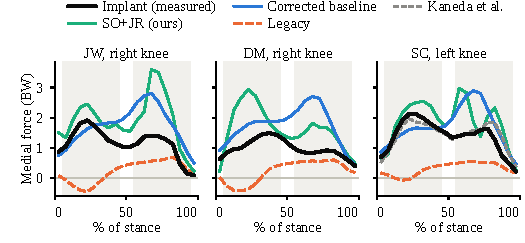
\includegraphics[width=\columnwidth]{figures/fig2_invivo.pdf}
\caption{Medial force against the implants: means of instrumented-limb stance frames in 5\%
bins (physical sign; SC only in Kaneda et al.'s windows). Corrected: 3-seed ensemble.
Legacy: optimizer-point model. Shading: peak windows.}
\label{fig:invivo}
\end{figure}

\subsection{Input Construction (D4)}\label{sec:res-d4}
The legacy builder sampled the position windows on an even grid over the whole IK segment,
including the 0.3-s SO buffers, while joint angles, flags and labels sat on the JR frames. On an
8-s Carter trial this shifted positions against labels by $-0.300$ to $+0.304$~s (mean
absolute 0.151~s), and on a Moore and a Lencioni trial by up to 0.18 and 0.075~s. The builder also
kept each lab's native rate (100--250~Hz), so a 20-frame window spanned 80~ms on Carter trials
(80.6\% of training frames) but 200~ms on Moore trials and in deployment. The test features shared
the warp, so held-out scores could not reveal it.

\subsection{In Vivo Medial Force}\label{sec:res-invivo}
SO+JR over-reads medial force (MAE 0.64--0.66~BW; Table~\ref{tab:invivo}, Fig.~\ref{fig:invivo}).
It has the double hump, but its early peaks are too high by 0.58--1.35~BW and its late peaks by
1.64 (SC) and 2.92~BW (JW) (3--6 windows per knee and half). Its medial share of axial force
(0.54--0.61) matches the implant's (0.48--0.71), so the excess is in the total force. On the same SC frames, Kaneda et al.'s released SO+JR reaches an MAE of 0.28~BW,
against 0.61~BW for ours. Stored labels and legacy surrogates miss the early peak by 1.14--1.51
and 1.2--1.6~BW.

% ---------------------------------------------------------------------------------------------
\begin{table}[t]
\caption{Held-Out Accuracy and Sensitivity}
\label{tab:sens}
\centering\footnotesize
\setlength{\tabcolsep}{3pt}
\begin{tabular}{@{}lcc@{}}
\toprule
Quantity & Legacy & Corrected\\
\midrule
Held-out $\Fmed$ MAE (BW)                 & 1.26 & 0.43--0.44\\
Held-out $\Fmed$ $r$                      & 0.46 & 0.70--0.77\\
Stance-peak error (BW)                    & $-2.02$ & $-0.86$ to $-0.81$\\
Limit recall / precision                  & 0.003 / 0.64 & 0.70--0.98 / 0.81--0.91\\
S1: recall, $\phi$--$d$ grid              & 0.001--0.005 & 0.49--0.99\\
S2: foot-point swap$^a$ (BW)              & 0.019 & 0.019\\
S2: pelvis angles$^b$ (BW)                & $+0.11$ & $-0.05$ to $-0.01$\\
S3: training $\to$ aligned$^c$ (BW)       & 1.13 $\to$ 1.10 & --\\
S4: reference, stance-1 mean (BW)         & 0.26 & 1.80--2.45\\
S4: reference, stance $>$1.4~BW (\%)      & 0 & 100\\
Xsens: IMU vs optical$^d$ (BW)            & -- & 0.38\\
\bottomrule
\end{tabular}\\[2pt]
\parbox{\columnwidth}{\scriptsize Physical sign throughout. Held-out rows: right-knee walking
stance frames of the test split with quality-checked SO+JR labels (33,915 frames of five people,
93\% from one Moore person); aligned inputs. Legacy: optimizer-point model. Corrected: range over
seeds 1--3; their ensemble (averaged predictions) beats each seed: MAE 0.41, $r$ 0.78, peak error
$-0.85$, recall 0.87, precision 0.84. $^a$Median absolute change of trial MAE, 605 trials (seed 1
vs.\ 3: 0.023); the legacy pair also differ in training run. $^b$Mean change of the reference
stance reading when pelvis angles are converted. $^c$In vivo MAE, JW. $^d$$\Fmed$ MAE, all
frames, median over 9 people; ensemble of seeds 1 and 3 (damped seed 2: 0.27; all three: 0.33);
static calibration, gyro contact.}
\end{table}

\subsection{Sensitivity}\label{sec:res-sens}
\textit{S1.} The constants trade off against label bias. Against the implants, SO+JR fits best
at the grid corner ($\phi = 0.4$, $d = 50$~mm) in all three subjects (MAE 0.40--0.52~BW, against
0.64--0.66~BW at the nominal values), still over-reading by 0.14--0.29~BW; the stored labels fit
best at $\phi = 0.6$. The same 1.4~BW limit therefore marks different loads for different label
sources. On the test split, the share of limit crossings that the seeds catch varies widely over
the grid (Table~\ref{tab:sens}).

\textit{S2.} The foot point changes held-out accuracy no more than swapping seeds does
(Table~\ref{tab:sens}). The converter we used to prepare the optimizer's reference motion for
OpenSim copies its pelvis angles, which rotate about other axes, into OpenSim's pelvis coordinates
(errors up to 12.9$^\circ$ in stance). Converting them barely moves the corrected readings of that
motion, but there the calcaneus-origin run reads 0.30~BW above seed~1, outside the seed range in
77\% of stance frames.

\textit{S3.} Scored in vivo, aligning the legacy inputs changes their error by at most 0.03~BW
(Table~\ref{tab:sens}).

% ---------------------------------------------------------------------------------------------
\begin{figure}[t]
\centering
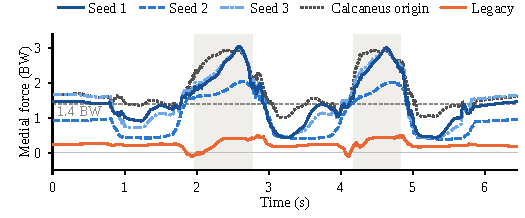
\includegraphics[width=\columnwidth]{figures/fig_sep23_seeds.pdf}
\caption{$\Fmed$ on the locked-knee reference motion of the optimizer of \Chong{}~\citeChong{},
which has no usable labels (same inputs for every model, pelvis angles converted; physical sign).
Legacy: optimizer-point model. Shading: right single stance. Dashed: 1.4~BW limit.}
\label{fig:refmotion}
\end{figure}

\textit{S4.} The SO+JR labels of the reference motion are unusable. Its COP stays at the
optimizer's mid-foot contact point through every single stance, which alone makes the fixed-COP rule
remove every right-knee frame; the copied pelvis angles (S2) also place the scaled model's foot
11.0~cm on average from the applied COP, an effect on the labels we did not test. We therefore
compare the models with each other (Fig.~\ref{fig:refmotion}). Read with the physical sign, every corrected run exceeds 1.4~BW in every
frame of both right single stances, and both legacy models stay below it (Table~\ref{tab:sens});
with their (inverted) training sign, the legacy models read stance-1 means of 0.79--1.04 and
peaks of 1.66--2.04~BW. Corrected and legacy models thus fall on opposite sides
of the limit, and without labels nothing on this motion shows which side is right. The seeds agree
on the verdict but not on the load: their per-frame range averages 0.73 and reaches 1.02~BW,
mostly due to seed~2.

\subsection{Corrected Baseline}\label{sec:res-corrected}
On held-out walking, the corrected seeds track SO+JR far more closely than the legacy model, which
learned the stored labels (Table~\ref{tab:sens}); the labels exceed 1.4~BW in 70\% of these
stance frames, and the seeds catch most of these crossings, the legacy model almost none. In vivo
(Table~\ref{tab:invivo}, Fig.~\ref{fig:invivo}), the baseline correlates positively in all three
knees, where the legacy models anti-correlate. But it inherits the over-read of its labels, has
one late hump at 60--70\% of stance instead of two, and tracks the implants less well than its
labels, also on quality-checked frames (JW $r$ 0.41 vs.\ 0.87, SC 0.47 vs.\ 0.74). Seeds with
equal pooled held-out error (person means 0.48, 0.63 and 0.52~BW) do not tie elsewhere: seed~2
flags the most crossings (recall 0.98, but precision 0.81) and is closest to the implants in every
knee (SC late peak $+0.31$ vs.\ $+1.55$ and $+1.60$~BW), yet reads the reference motion lowest.

\subsection{Wearable Path}\label{sec:res-wearable}
On the simulated suit (two held-out trials, 1$^\circ$ noise), the worst joint-angle
root-mean-square error (RMSE) was 2.1$^\circ$ and 1.8$^\circ$. Contact detection, not orientation
noise, drove the deviation of $\Fmed$ from the same surrogate fed with mocap: in stance 0.16 and
0.22~BW with the gyro detector against 0.07 and 0.06~BW with force-plate contact (seed~1; gyro
seed means 0.12 and 0.18). Back-dating cut the deviation from 0.24 to 0.16~BW on one trial
but only from 0.23 to 0.22~BW on the
other, where the detector re-triggered in 3 of 11 left swings, and it left the error against
quality-checked labels unchanged (0.43~BW, seed~1). A full driver frame
costs about 2.4~ms on one CPU thread, well within the 16.7-ms suit period.

On the 54 Xsens trials of 9 people, the UKF's right knee angle differed from optical IK by a median
per-person RMSE of 5.0$^\circ$ (mostly a $-3.5^\circ$ offset), against 2.2$^\circ$ for the vendor's
angles. $\Fmed$ on IMU input differed from that on optical input (Table~\ref{tab:sens})
mostly through contact: with treadmill contact flags the difference was
0.14~BW. The gyro detector agreed with the treadmill in only 0.64--0.73 of frames below 1.25~m/s,
against 0.84--0.86 at 1.25--1.50~m/s, where the difference fell to about 0.2~BW; in a pilot, the
swing foot turned at only 150--320$^\circ$/s at 0.25--0.75~m/s, below the 400$^\circ$/s release
threshold.

% discussion.tex -- Sections V and VI. Sources as in results.tex. Facts about Chong et al.:
% the published text describes SO+JR labels and states that M_add > 0 loads the medial
% compartment (paper/author.tex lines 537, 554); its reductions were not checked with SO+JR
% (ISRR2). Kaneda 0.28 BW = our recomputation on SC (gc/pilot_AB_sojr/README.md); "5 of 94
% segments cover a full stance" (qc_final.md fix:label-qc open issues).
% "Cannot confirm or refute" rests on D1 and D2, which hold for every checkpoint trained on the stored
% labels and for every optimizer run that forms the proxy with +M_x at the right knee, NOT on the in
% vivo r of the two audited checkpoints: which checkpoint produced the figures of [4] is unconfirmed
% (facts ISRR4; TODO before submission: confirm with the first author). SC residual over-read:
% audit_gc/qc_keep/summary.csv; 25.4 %: labels_qc/label_masks/by_lab.csv (see results.tex).
% Moore share: 92.6 % of QC-passing training frames (labels_qc/label_masks/dry_build_fpopt/
% kept_by_lab.csv, 327,287 / 353,581) and 92.9 % of held-out stance frames (fmedial_eval/
% audit_test_qc/summary.csv, 31,515 / 33,915). Optimizer input convention for the pelvis angles is
% unverified (sep23/README.md; evals_final.md fix:sep23). The reference motion's COP is pinned at the optimizer's
% contact point, which alone fails the fixed-COP rule (sep23/README.md), so verifying synthesized gaits needs a
% moving COP as well as converted pelvis angles. Test split: one person per lab (fmedial_eval/audit_test_qc).
\section{Discussion}\label{sec:discussion}
\textit{What the audit means for the optimizer.} \Chong{}~\citeChong{} describe SO+JR labels
and a medial-positive moment, but the stored labels lack the SO muscle forces (D1) and the
inference code uses the inverted sign (D2). D1 affects every checkpoint trained on the stored
labels and D2 every optimizer run with this proxy, whichever checkpoint it queried; held-out
accuracy hid both, because training and test labels share them. The reported load reductions are
surrogate predictions not checked with SO+JR, so this audit can neither confirm nor refute them,
and the in vivo scores of the two audited checkpoints need not carry over to others. On the
optimizer's reference motion, corrected and legacy models fall on opposite sides of the limit.
Running SO+JR on the synthesized gaits, with converted pelvis angles and a moving COP, would test in
the model whether they unload the knee; in vivo confirmation needs measurement.

\textit{Neither label source is ground truth.} The stored labels are too low and the SO+JR
labels too high. The quality rules remove the worst of D3 but keep only a quarter of stance time
and little of Carter or Lencioni, and frames that pass them are still over-read in all three knees
(Sec.~\ref{sec:res-d3}); the corrected baseline inherits this. On SC, Kaneda et al.'s SO+JR, with
separate medial and lateral contacts, fitted the implant far better (Sec.~\ref{sec:res-invivo}),
so SO+JR can do better than our labels; their contact model may explain the difference.
Re-solving SO per frame and repairing the COP would keep more data.

\textit{Recommendations.} For learned models whose outputs act on people: (i)~check that the physics ran
as described (D1); (ii)~test sign and axis conventions on a case with a known answer (D2, S2);
(iii)~compare label magnitudes with in vivo data (D3); (iv)~build features with the deployment
code (D4); (v)~report seed spread off the training distribution, and verify optimized motions
with physics before they reach a patient.

\textit{Social impact.} Gait retraining has lowered KAM and pain~\cite{shull2013six}, and a
wearable surrogate could take pain-aware coaching out of the lab once contact detection works in
slow walking and its loads agree with in vivo measurement. The main risk is false reassurance: an under-reading model certifies a harmful gait as
safe, while an over-reading one steers patients toward needless changes. $\Fmed$ remains a proxy, and medial load is not pain, so patient use
also needs clinical validation.

\textit{Limitations.} The in vivo subjects are three knee-replacement patients, not OA knees; most
segments cover only half a stance, peak errors rest on 3--6 windows per knee and half, and DM's
timing is uncertain. Our SO+JR uses a single knee contact. The 40 peaks were hand-picked, so their
causes are not prevalences. The test split has one person per lab; Moore supplies 93\% of the
quality-checked training frames, and one Moore person 93\% of the held-out frames. The optimizer
was not available, so its pelvis-angle convention is unverified, and S1 is not propagated through
it (future work). The real-sensor data have no knee-load labels, and the suit's label error rests
on one trial.

\section{Conclusion}\label{sec:conclusion}
A learned pain-risk surrogate inherits the defects of its label pipeline and input construction,
and held-out accuracy hides those that the test data share. Auditing one such pipeline against
physics, instrumented knees and its own code found four defects. Retrained on quality-checked
labels with the physical sign, the surrogate correlates positively with the implants but less well
than its labels; on the optimizer's reference motion its seeds agree on the verdict but differ by
up to 1.0~BW in load. A load reduction found by optimizing such a
surrogate is a hypothesis to verify with physics.


\bibliographystyle{IEEEtran}
\bibliography{refs}

\end{document}
